
%% bare_conf.tex
%% V1.3
%% 2007/01/11
%% by Michael Shell
%% See:
%% http://www.michaelshell.org/
%% for current contact information.
%%
%% This is a skeleton file demonstrating the use of IEEEtran.cls
%% (requires IEEEtran.cls version 1.7 or later) with an IEEE conference paper.
%%
%% Support sites:
%% http://www.michaelshell.org/tex/ieeetran/
%% http://www.ctan.org/tex-archive/macros/latex/contrib/IEEEtran/
%% and
%% http://www.ieee.org/

%%*************************************************************************
%% Legal Notice:
%% This code is offered as-is without any warranty either expressed or
%% implied; without even the implied warranty of MERCHANTABILITY or
%% FITNESS FOR A PARTICULAR PURPOSE! 
%% User assumes all risk.
%% In no event shall IEEE or any contributor to this code be liable for
%% any damages or losses, including, but not limited to, incidental,
%% consequential, or any other damages, resulting from the use or misuse
%% of any information contained here.
%%
%% All comments are the opinions of their respective authors and are not
%% necessarily endorsed by the IEEE.
%%
%% This work is distributed under the LaTeX Project Public License (LPPL)
%% ( http://www.latex-project.org/ ) version 1.3, and may be freely used,
%% distributed and modified. A copy of the LPPL, version 1.3, is included
%% in the base LaTeX documentation of all distributions of LaTeX released
%% 2003/12/01 or later.
%% Retain all contribution notices and credits.
%% ** Modified files should be clearly indicated as such, including  **
%% ** renaming them and changing author support contact information. **
%%
%% File list of work: IEEEtran.cls, IEEEtran_HOWTO.pdf, bare_adv.tex,
%%                    bare_conf.tex, bare_jrnl.tex, bare_jrnl_compsoc.tex
%%*************************************************************************

% *** Authors should verify (and, if needed, correct) their LaTeX system  ***
% *** with the testflow diagnostic prior to trusting their LaTeX platform ***
% *** with production work. IEEE's font choices can trigger bugs that do  ***
% *** not appear when using other class files.                            ***
% The testflow support page is at:
% http://www.michaelshell.org/tex/testflow/



% Note that the a4paper option is mainly intended so that authors in
% countries using A4 can easily print to A4 and see how their papers will
% look in print - the typesetting of the document will not typically be
% affected with changes in paper size (but the bottom and side margins will).
% Use the testflow package mentioned above to verify correct handling of
% both paper sizes by the user's LaTeX system.
%
% Also note that the "draftcls" or "draftclsnofoot", not "draft", option
% should be used if it is desired that the figures are to be displayed in
% draft mode.
%
\documentclass[10pt, conference, compsocconf]{IEEEtran}
% Add the compsocconf option for Computer Society conferences.
%
% If IEEEtran.cls has not been installed into the LaTeX system files,
% manually specify the path to it like:
% \documentclass[conference]{../sty/IEEEtran}

\usepackage{graphicx}
\usepackage[nosectionbib]{apacite}
\usepackage{natbib}
\usepackage{amsmath}
\usepackage{cite}
\usepackage{apacite}
% Some very useful LaTeX packages include:
% (uncomment the ones you want to load)


% *** MISC UTILITY PACKAGES ***
%
%\usepackage{ifpdf}
% Heiko Oberdiek's ifpdf.sty is very useful if you need conditional
% compilation based on whether the output is pdf or dvi.
% usage:
% \ifpdf
%   % pdf code
% \else
%   % dvi code
% \fi
% The latest version of ifpdf.sty can be obtained from:
% http://www.ctan.org/tex-archive/macros/latex/contrib/oberdiek/
% Also, note that IEEEtran.cls V1.7 and later provides a builtin
% \ifCLASSINFOpdf conditional that works the same way.
% When switching from latex to pdflatex and vice-versa, the compiler may
% have to be run twice to clear warning/error messages.






% *** CITATION PACKAGES ***
%
%\usepackage{cite}
% cite.sty was written by Donald Arseneau
% V1.6 and later of IEEEtran pre-defines the format of the cite.sty package
% \cite{} output to follow that of IEEE. Loading the cite package will
% result in citation numbers being automatically sorted and properly
% "compressed/ranged". e.g., [1], [9], [2], [7], [5], [6] without using
% cite.sty will become [1], [2], [5]--[7], [9] using cite.sty. cite.sty's
% \cite will automatically add leading space, if needed. Use cite.sty's
% noadjust option (cite.sty V3.8 and later) if you want to turn this off.
% cite.sty is already installed on most LaTeX systems. Be sure and use
% version 4.0 (2003-05-27) and later if using hyperref.sty..sty does
% not currently provide for hyperlinked citations.
% The latest version can be obtained at:
% http://www.ctan.org/tex-archive/macros/latex/contrib/cite/
% The documentation is contained in the cite.sty file itself.






% *** GRAPHICS RELATED PACKAGES ***
%
\ifCLASSINFOpdf
  % \usepackage[pdftex]{graphicx}
  % declare the path(s) where your graphic files are
  % \graphicspath{{../pdf/}{../jpeg/}}
  % and their extensions so you won't have to specify these with
  % every instance of \includegraphics
  % \DeclareGraphicsExtensions{.pdf,.jpeg,.png}
\else
  % or other class option (dvipsone, dvipdf, if not using dvips). graphicx
  % will default to the driver specified in the system graphics.cfg if no
  % driver is specified.
   %\usepackage[dvips]{graphicx}
  % declare the path(s) where your graphic files are
  % \graphicspath{{../eps/}}
  % and their extensions so you won't have to specify these with
  % every instance of \includegraphics
  % \DeclareGraphicsExtensions{.eps}
\fi
% graphicx was written by David Carlisle and Sebastian Rahtz. It is
% required if you want graphics, photos, etc. graphicx.sty is already
% installed on most LaTeX systems. The latest version and documentation can
% be obtained at: 
% http://www.ctan.org/tex-archive/macros/latex/required/graphics/
% Another good source of documentation is "Using Imported Graphics in
% LaTeX2e" by Keith Reckdahl which can be found as epslatex.ps or
% epslatex.pdf at: http://www.ctan.org/tex-archive/info/
%
% latex, and pdflatex in dvi mode, support graphics in encapsulated
% postscript (.eps) format. pdflatex in pdf mode supports graphics
% in .pdf, .jpeg, .png and .mps (metapost) formats. Users should ensure
% that all non-photo figures use a vector format (.eps, .pdf, .mps) and
% not a bitmapped formats (.jpeg, .png). IEEE frowns on bitmapped formats
% which can result in "jaggedy"/blurry rendering of lines and letters as
% well as large increases in file sizes.
%
% You can find documentation about the pdfTeX application at:
% http://www.tug.org/applications/pdftex





% *** MATH PACKAGES ***
%
%\usepackage[cmex10]{amsmath}
% A popular package from the American Mathematical Society that provides
% many useful and powerful commands for dealing with mathematics. If using
% it, be sure to load this package with the cmex10 option to ensure that
% only type 1 fonts will utilized at all point sizes. Without this option,
% it is possible that some math symbols, particularly those within
% footnotes, will be rendered in bitmap form which will result in a
% document that can not be IEEE Xplore compliant!
%
% Also, note that the amsmath package sets \interdisplaylinepenalty to 10000
% thus preventing page breaks from occurring within multiline equations. Use:
%\interdisplaylinepenalty=2500
% after loading amsmath to restore such page breaks as IEEEtran.cls normally
% does. amsmath.sty is already installed on most LaTeX systems. The latest
% version and documentation can be obtained at:
% http://www.ctan.org/tex-archive/macros/latex/required/amslatex/math/





% *** SPECIALIZED LIST PACKAGES ***
%
%\usepackage{algorithmic}
% algorithmic.sty was written by Peter Williams and Rogerio Brito.
% This package provides an algorithmic environment fo describing algorithms.
% You can use the algorithmic environment in-text or within a figure
% environment to provide for a floating algorithm. Do NOT use the algorithm
% floating environment provided by algorithm.sty (by the same authors) or
% algorithm2e.sty (by Christophe Fiorio) as IEEE does not use dedicated
% algorithm float types and packages that provide these will not provide
% correct IEEE style captions. The latest version and documentation of
% algorithmic.sty can be obtained at:
% http://www.ctan.org/tex-archive/macros/latex/contrib/algorithms/
% There is also a support site at:
% http://algorithms.berlios.de/index.html
% Also of interest may be the (relatively newer and more customizable)
% algorithmicx.sty package by Szasz Janos:
% http://www.ctan.org/tex-archive/macros/latex/contrib/algorithmicx/


%\usepackage{harvard}
%\usepackage[backend=bibtex]{bib latex}

% *** ALIGNMENT PACKAGES ***
%
%\usepackage{array}
% Frank Mittelbach's and David Carlisle's array.sty patches and improves
% the standard LaTeX2e array and tabular environments to provide better
% appearance and additional user controls. As the default LaTeX2e table
% generation code is lacking to the point of almost being broken with
% respect to the quality of the end results, all users are strongly
% advised to use an enhanced (at the very least that provided by array.sty)
% set of table tools. array.sty is already installed on most systems. The
% latest version and documentation can be obtained at:
% http://www.ctan.org/tex-archive/macros/latex/required/tools/


%\usepackage{mdwmath}
%\usepackage{mdwtab}
% Also highly recommended is Mark Wooding's extremely powerful MDW tools,
% especially mdwmath.sty and mdwtab.sty which are used to format equations
% and tables, respectively. The MDWtools set is already installed on most
% LaTeX systems. The lastest version and documentation is available at:
% http://www.ctan.org/tex-archive/macros/latex/contrib/mdwtools/


% IEEEtran contains the IEEEeqnarray family of commands that can be used to
% generate multiline equations as well as matrices, tables, etc., of high
% quality.


%\usepackage{eqparbox}
% Also of notable interest is Scott Pakin's eqparbox package for creating
% (automatically sized) equal width boxes - aka "natural width parboxes".
% Available at:
% http://www.ctan.org/tex-archive/macros/latex/contrib/eqparbox/





% *** SUBFIGURE PACKAGES ***
%\usepackage[tight,footnotesize]{subfigure}
% subfigure.sty was written by Steven Douglas Cochran. This package makes it
% easy to put subfigures in your figures. e.g., "Figure 1a and 1b". For IEEE
% work, it is a good idea to load it with the tight package option to reduce
% the amount of white space around the subfigures. subfigure.sty is already
% installed on most LaTeX systems. The latest version and documentation can
% be obtained at:
% http://www.ctan.org/tex-archive/obsolete/macros/latex/contrib/subfigure/
% subfigure.sty has been superceeded by subfig.sty.



%\usepackage[caption=false]{caption}
%\usepackage[font=footnotesize]{subfig}
% subfig.sty, also written by Steven Douglas Cochran, is the modern
% replacement for subfigure.sty. However, subfig.sty requires and
% automatically loads Axel Sommerfeldt's caption.sty which will override
% IEEEtran.cls handling of captions and this will result in nonIEEE style
% figure/table captions. To prevent this problem, be sure and preload
% caption.sty with its "caption=false" package option. This is will preserve
% IEEEtran.cls handing of captions. Version 1.3 (2005/06/28) and later 
% (recommended due to many improvements over 1.2) of subfig.sty supports
% the caption=false option directly:
%\usepackage[caption=false,font=footnotesize]{subfig}
%
% The latest version and documentation can be obtained at:
% http://www.ctan.org/tex-archive/macros/latex/contrib/subfig/
% The latest version and documentation of caption.sty can be obtained at:
% http://www.ctan.org/tex-archive/macros/latex/contrib/caption/




% *** FLOAT PACKAGES ***
%
%\usepackage{fixltx2e}
% fixltx2e, the successor to the earlier fix2col.sty, was written by
% Frank Mittelbach and David Carlisle. This package corrects a few problems
% in the LaTeX2e kernel, the most notable of which is that in current
% LaTeX2e releases, the ordering of single and double column floats is not
% guaranteed to be preserved. Thus, an unpatched LaTeX2e can allow a
% single column figure to be placed prior to an earlier double column
% figure. The latest version and documentation can be found at:
% http://www.ctan.org/tex-archive/macros/latex/base/



%\usepackage{stfloats}
% stfloats.sty was written by Sigitas Tolusis. This package gives LaTeX2e
% the ability to do double column floats at the bottom of the page as well
% as the top. (e.g., "\begin{figure*}[!b]" is not normally possible in
% LaTeX2e). It also provides a command:
%\fnbelowfloat
% to enable the placement of footnotes below bottom floats (the standard
% LaTeX2e kernel puts them above bottom floats). This is an invasive package
% which rewrites many portions of the LaTeX2e float routines. It may not work
% with other packages that modify the LaTeX2e float routines. The latest
% version and documentation can be obtained at:
% http://www.ctan.org/tex-archive/macros/latex/contrib/sttools/
% Documentation is contained in the stfloats.sty comments as well as in the
% presfull.pdf file. Do not use the stfloats baselinefloat ability as IEEE
% does not allow \baselineskip to stretch. Authors submitting work to the
% IEEE should note that IEEE rarely uses double column equations and
% that authors should try to avoid such use. Do not be tempted to use the
% cuted.sty or midfloat.sty packages (also by Sigitas Tolusis) as IEEE does
% not format its papers in such ways.





% *** PDF, URL AND HYPERLINK PACKAGES ***
%
%\usepackage{url}
% url.sty was written by Donald Arseneau. It provides better support for
% handling and breaking URLs. url.sty is already installed on most LaTeX
% systems. The latest version can be obtained at:
% http://www.ctan.org/tex-archive/macros/latex/contrib/misc/
% Read the url.sty source comments for usage information. Basically,
% \url{my_url_here}.





% *** Do not adjust lengths that control margins, column widths, etc. ***
% *** Do not use packages that alter fonts (such as pslatex).         ***
% There should be no need to do such things with IEEEtran.cls V1.6 and later.
% (Unless specifically asked to do so by the journal or conference you plan
% to submit to, of course. )


% correct bad hyphenation here
\hyphenation{op-tical net-works semi-conduc-tor}


\begin{document}
%
% paper title
% can use linebreaks \\ within to get better formatting as desired
\title{Bare Demo of IEEEtran.cls for IEEECS Conferences}


% author names and affiliations
% use a multiple column layout for up to two different
% affiliations

\author{Ye Zhang}

% conference papers do not typically use \thanks and this command
% is locked out in conference mode. If really needed, such as for
% the acknowledgment of grants, issue a \IEEEoverridecommandlockouts
% after \documentclass

% for over three affiliations, or if they all won't fit within the width
% of the page, use this alternative format:
% 
%\author{\IEEEauthorblockN{Michael Shell\IEEEauthorrefmark{1},
%Homer Simpson\IEEEauthorrefmark{2},
%James Kirk\IEEEauthorrefmark{3}, 
%Montgomery Scott\IEEEauthorrefmark{3} and
%Eldon Tyrell\IEEEauthorrefmark{4}}
%\IEEEauthorblockA{\IEEEauthorrefmark{1}School of Electrical and Computer Engineering\\
%Georgia Institute of Technology,
%Atlanta, Georgia 30332--0250\\ Email: see http://www.michaelshell.org/contact.html}
%\IEEEauthorblockA{\IEEEauthorrefmark{2}Twentieth Century Fox, Springfield, USA\\
%Email: homer@thesimpsons.com}
%\IEEEauthorblockA{\IEEEauthorrefmark{3}Starfleet Academy, San Francisco, California 96678-2391\\
%Telephone: (800) 555--1212, Fax: (888) 555--1212}
%\IEEEauthorblockA{\IEEEauthorrefmark{4}Tyrell Inc., 123 Replicant Street, Los Angeles, California 90210--4321}}




% use for special paper notices
%\IEEEspecialpapernotice{(Invited Paper)}




% make the title area
\maketitle


\begin{abstract}
In California Department of Motor Vehicles(DMV),  people sometimes have to waiting a long time to get services. It is necessary to anticipate future waiting time based on history so that
people can choose a better time and a better nearby DMV office. This paper evaluates future waiting time prediction methods: hidden Markov model, dynamic Bayesian network, Markov chain model, n-gram language model,
decision tree and support vector machine(SVM). We calculate the average prediction error in hours to compare these different models. 
\end{abstract}

\begin{IEEEkeywords}
component; formatting; style; styling;

\end{IEEEkeywords}


% For peer review papers, you can put extra information on the cover
% page as needed:
% \ifCLASSOPTIONpeerreview
% \begin{center} \bfseries EDICS Category: 3-BBND \end{center}
% \fi
%
% For peerreview papers, this IEEEtran command inserts a page break and
% creates the second title. It will be ignored for other modes.
\IEEEpeerreviewmaketitle



\section{Introduction}
% no \IEEEPARstart
Can future waiting time be predicted based on previous waiting time in DMV office? Normally, waiting time in an office follows some regular patterns. For example, if there is long queue at 11:00 am in a certain
DMV, there might be also a long queue at 11:10 am in this office. Also, we observe that people prefer to go to DMV late in the morning or early in the afternoon rather than
early in the morning or late in the afternoon. So if a person asks when he should go to DMV best, we might suggest that he should choose early in the morning or late in the afternoon.
However, sometimes, people are not available in these time buckets and they have to go to DMV  during peak hours. In this case, we have to think of some methods to predict waiting time at a certain time
in the future when people want to go to DMV to better satisfy their needs. 

In this paper, we predict future waiting time based on previous waiting time and corresponding time buckets. We use "DMV
office waiting time" dataset. In this dataset, we have waiting time in 176 DMV offices in recent 3 months. The waiting time for each office is sampled one time every 10 minutes, so we use 10 minutes as 
a time bucket. For example, between 8:00 am and 9:00 am, we have 8:00--8:10, 8:10--8:20, 8:20--8:30, 8:30--8:40, 8:40--8:50, 8:50--9:00 these time buckets, and other time is similar. Several prediction techniques
are proposed in this paper including hidden Markov model(HMM), dynamic Bayesian model, Markov chain model, n-gram language model, decision tree and SVM. We split the whole dataset into two parts
with equal size. One is used for training and the other is used for testing. Continuous waiting time in training dataset is discretized into 20 discrete values which we use to denote different states. This is obtained by drawing equal height histogram for all waiting time values for the office. In this histogram, we have 20 intervals and in each bucket, we have the same number of values of waiting time. Then we use the median value of each interval to denote the discrete value for all the waiting time values that in this interval.

The main criterion for
comparison is the average prediction error. After we use different models to train the dataset, we predict a discrete value for a given future time bucket in the testing data and then convert this discrete value into corresponding continuous waiting time and compare this prediction value with the true waiting time. Finally, we compute average error over all testing data. 


% You must have at least 2 lines in the paragraph with the drop letter
% (should never be an issue)

\subsection{Subsection Heading Here}
Subsection text here.


\subsubsection{Subsubsection Heading Here}
Subsubsection text here.

\section{Related Work}
Some previous work has involved time series prediction.  \cite{4840324} has used HMM for modeling time series data.  

%Wherever Times is specified, Times Roman or Times New Roman may be used. If neither is available on your system, please use the font closest in appearance to Times. Avoid using bit-mapped fonts if possible. True-Type 1 %or Open Type fonts are preferred. Please embed symbol fonts, as well, for math, etc.
% An example of a floating figure using the graphicx package.
% Note that \label must occur AFTER (or within) \caption.
% For figures, \caption should occur after the \includegraphics.
% Note that IEEEtran v1.7 and later has special internal code that
% is designed to preserve the operation of \label within \caption
% even when the captionsoff option is in effect. However, because
% of issues like this, it may be the safest practice to put all your
% \label just after \caption rather than within \caption{}.
%
% Reminder: the "draftcls" or "draftclsnofoot", not "draft", class
% option should be used if it is desired that the figures are to be
% displayed while in draft mode.
%
%\begin{figure}[!t]
%\centering
%\includegraphics[width=2.5in]{myfigure}
% where an .eps filename suffix will be assumed under latex, 
% and a .pdf suffix will be assumed for pdflatex; or what has been declared
% via \DeclareGraphicsExtensions.
%\caption{Simulation Results}
%\label{fig_sim}
%\end{figure}

% Note that IEEE typically puts floats only at the top, even when this
% results in a large percentage of a column being occupied by floats.


% An example of a double column floating figure using two subfigures.
% (The subfig.sty package must be loaded for this to work.)
% The subfigure \label commands are set within each subfloat command, the
% \label for the overall figure must come after \caption.
% \hfil must be used as a separator to get equal spacing.
% The subfigure.sty package works much the same way, except \subfigure is
% used instead of \subfloat.
%
%\begin{figure*}[!t]
%\centerline{\subfloat[Case I]\includegraphics[width=2.5in]{subfigcase1}%
%\label{fig_first_case}}
%\hfil
%\subfloat[Case II]{\includegraphics[width=2.5in]{subfigcase2}%
%\label{fig_second_case}}}
%\caption{Simulation results}
%\label{fig_sim}
%\end{figure*}
%
% Note that often IEEE papers with subfigures do not employ subfigure
% captions (using the optional argument to \subfloat), but instead will
% reference/describe all of them (a), (b), etc., within the main caption.


% An example of a floating table. Note that, for IEEE style tables, the 
% \caption command should come BEFORE the table. Table text will default to
% \footnotesize as IEEE normally uses this smaller font for tables.
% The \label must come after \caption as always.
%
%\begin{table}[!t]
%% increase table row spacing, adjust to taste
%\renewcommand{\arraystretch}{1.3}
% if using array.sty, it might be a good idea to tweak the value of
% \extrarowheight as needed to properly center the text within the cells
%\caption{An Example of a Table}
%\label{table_example}
%\centering
%% Some packages, such as MDW tools, offer better commands for making tables
%% than the plain LaTeX2e tabular which is used here.
%\begin{tabular}{|c||c|}
%\hline
%One & Two\\
%\hline
%Three & Four\\
%\hline
%\end{tabular}
%\end{table}


% Note that IEEE does not put floats in the very first column - or typically
% anywhere on the first page for that matter. Also, in-text middle ("here")
% positioning is not used. Most IEEE journals/conferences use top floats
% exclusively. Note that, LaTeX2e, unlike IEEE journals/conferences, places
% footnotes above bottom floats. This can be corrected via the \fnbelowfloat
% command of the stfloats package.



\section{Prediction Models}
We developed and evaluated several statistical models to predict future waiting time without appointment at a certain office.
Since we sampled data each 10 minutes, we use 10 minutes as a time bucket.
We split the whole
dataset into two parts with equal size and use one for training and the other for testing. 
 In order to better visualize waiting time distribution, we choose three offices randomly among
all the offices and fit a Gaussian distribution for each time bucket for each of these three offices. We can see the distribution from
Figure \ref{Waiting Time for Office 504}, Figure \ref{Waiting Time for Office 548} and Figure \ref{Waiting Time for Office 632}.
Then we take into account waiting time values of all offices for each time bucket 
and again fit a Gaussian distribution for each time bucket. 

\begin{figure}[!t]
\centering
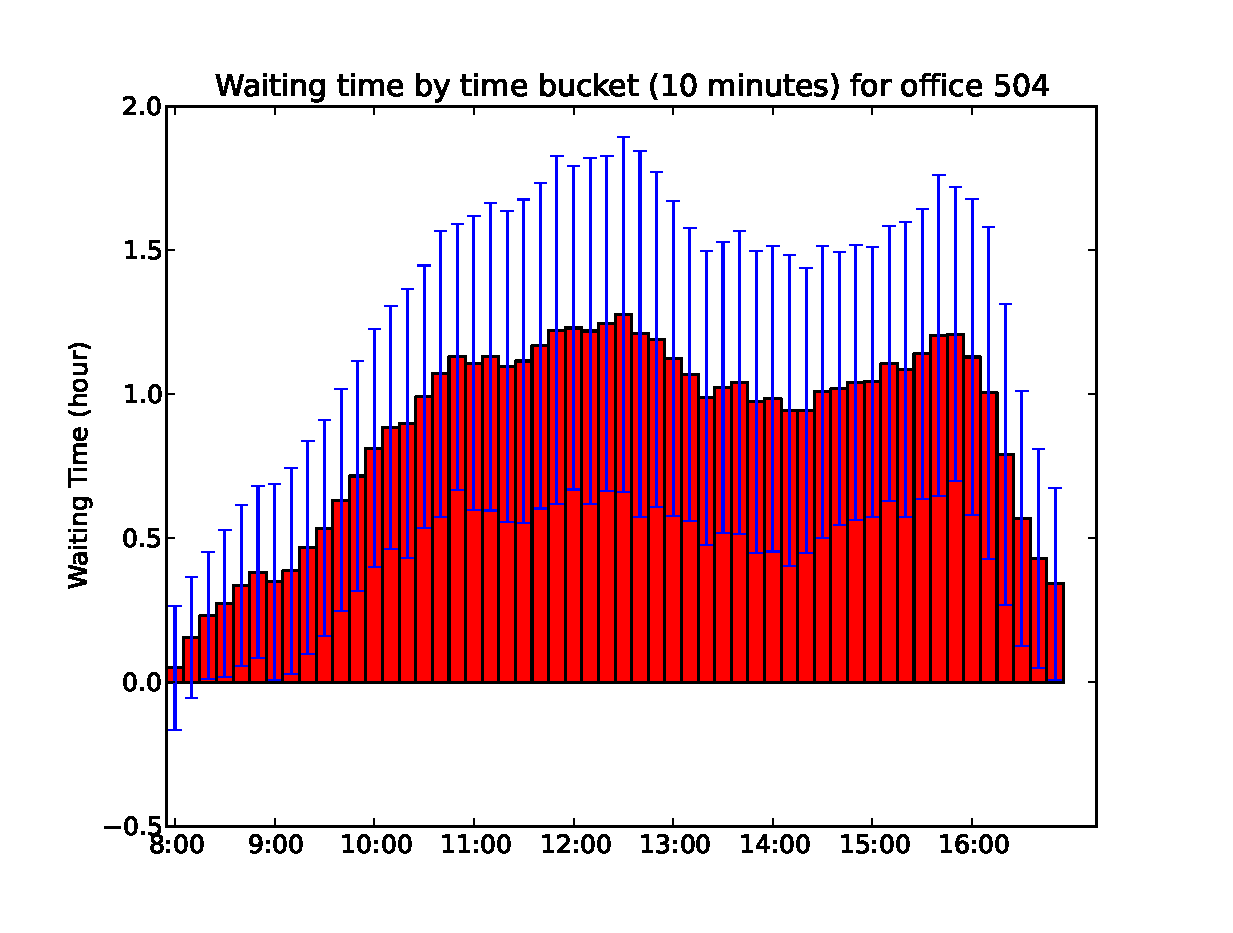
\includegraphics[width=3in]{Office504.eps}
\caption{Waiting Time Distribution for Office 504}
\label{Waiting Time for Office 504}
\end{figure}
\subsection{Time-based Waiting Time Prediction}

\begin{figure}[!t]
\centering
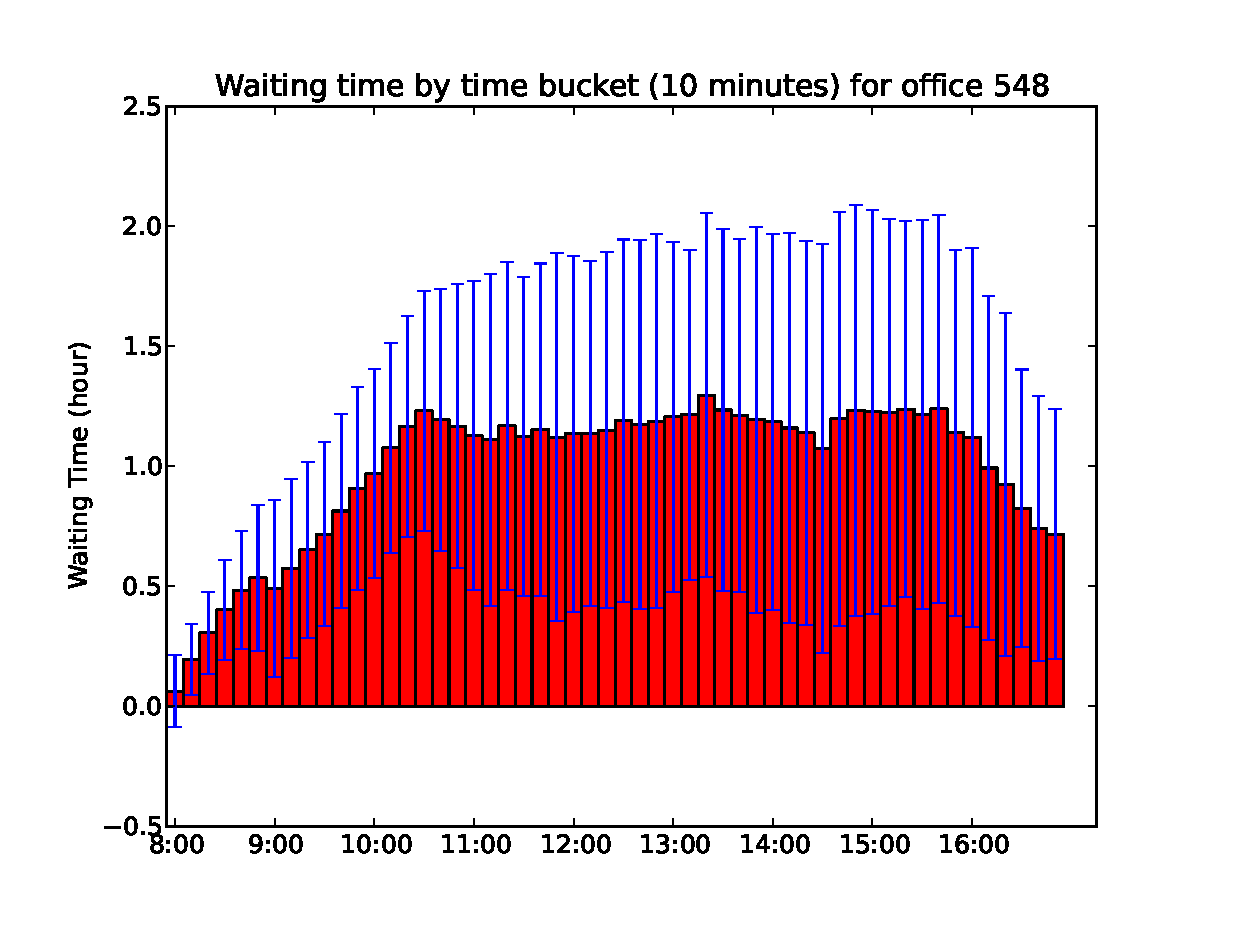
\includegraphics[width=3in]{Office548.eps}
\caption{Waiting Time Distribution for Office 548}
\label{Waiting Time for Office 548}
\end{figure}

\begin{figure}[!t]
\centering
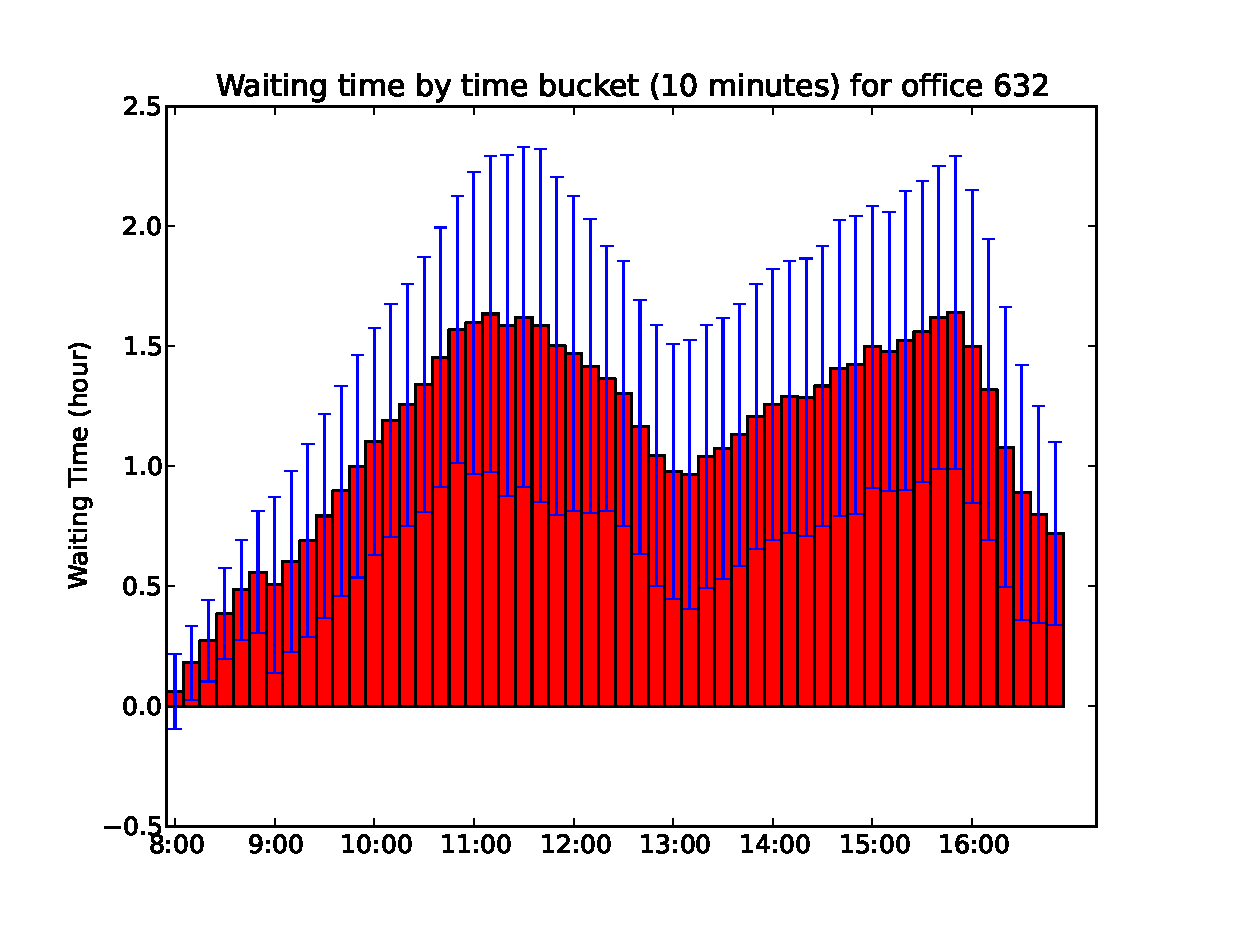
\includegraphics[width=3in]{Office632.eps}
\caption{Waiting Time Distribution for Office 632}
\label{Waiting Time for Office 632}
\end{figure}

\subsection{Time-based Waiting Time Prediction} first model used in our work is the time-based waiting time prediction model. This model uses only the time feature
to predict future waiting time.  and fit a Gaussian
distribution for each time bucket. The following is the error bar distribution for DMV office 632 whole complete day. We use the 
The average error over testing data is 0.5235 hour. 


%\begin{figure}[!t]
%\centering
%\includegraphics[width=2.5in]{myfigure}
% where an .eps filename suffix will be assumed under latex, 
% and a .pdf suffix will be assumed for pdflatex; or what has been declared
% via \DeclareGraphicsExtensions.
%\caption{Simulation Results}
%\label{fig_sim}
%\end{figure}



\subsection{HMM Model}
We use HMM to model time series. First we use MLE on training data to obtain transition probability, emission probability and
initial probability. Then we use Viterbi path algorithm to do inference on waiting time sequence given us a time sequence.
And we use this inferred waiting time sequence as prediction to calculate the error.
The error we obtained is 0.2981 hour. 

 \subsection{Danymic Bayesian Network}
We also use Danymic Bayesian Network to model the time series. The whole procedure is similar as in HMM model. But this time, we use weekday plus time of
day these two as two variables. So in total, there are three variables: waiting time, time of day, and weekday. We use MLE to
calculate necessary parameters including transition probability, emission probability and initial probability. Then we use Viterbi
algorithm to do inference on hidden sequence given a time sequence in testing data. The average error we obtained
is 0.7340 hour. So we can claim that after treating weekday as a feature, the prediction error will increase compared to HMM.

\subsection{One Order Markov Chain Model}
Actually, when we want to know waiting time at a given time bucket t, we always know waiting time at t-1plus prior knowledge about waiting
time at t.
Specifically, we want to calculate
\begin{equation}\label{OneOrderMarkovChain}
W_t=\underset{W_t}{\arg\max} {P(W_t|W_{t-1}, H_t)}
\end{equation}
where W\_t denotes the waiting time at time T, and H\_t denotes the time bucket. 

\subsubsection{Bayes Rule}
We first use Bayes rule to convert this formula to the following form assuming that H\_t is independent from transition probability :
\begin{equation}
W_t=\underset{W_t}{\arg\max} {P(W_{t-1}|W_t)*P(W_t|H_t)}
\end{equation}
We use MLE to calculate probability $P(W_{t-1}|W_t)$ and $P(W_t|H_t)$, and find the maximum $W_t$ for each given $H_t$
and $W_{t-1}$ in the testing data and use this maximum as prediction. The average error we obtain is 

\subsubsection{Log Linear Probability Model}
We use log linear model to obtain the following equation from equation \eqref{OneOrderMarkovChain}:
\begin{equation}
\begin{split}
W_t=\underset{W_t}{\arg\max}{\lambda*\log P(W_t|W_{t-1})+\ \
(1-\lambda)*\log P(W_t|H_t)}
\end{split}
\end{equation}
Still, we use MLE to obtain transition probability $P(W_t|W_{t-1})$ and try different $\lambda$ . The average error is 


\subsection{4-Gram Language Model}
In practice, when we want to predict next waiting time, we know not only previous moment's waiting time, but also previous waiting time of
several time buckets. So we try 4-Gram Language Model where we model each complete time sequence as a sentence in 4-Gram model.
The task is to predict a word (waiting time) at a location given previous three words (three time buckets' waiting time).
Then we use back-off model to do prediction on testing data. The average error is 

\subsection{Reversed 3-order Markov Model}
In the case where we know previous three time buckets' waiting time, we want:
\begin{equation}
\begin{split}
W_t=\underset{W_t}{\arg\max}{P(W_t|W_{t-1},W_{t-2},W_{t-3},H_t)} \\
=\underset{W_t}{\arg\max}{P(W_t,W_{t-1},W_{t-2},W_{t-3}}
=\underset{W_t}{\arg\max}{P(W_t|H_t)*P(W_{t-1}|W_t)*P(W_{t-2}|W_t,W_{t-1})*\ \
P(W_{t-3}|W_{t-2},W_{t-1},W_t)}
\end{split}
We reverse the waiting time sequence to W_n, W_n-1, \ldots W_3, W_2, W_1 and train an n-gram
back-off model from the reversed data. The error of this model is 
\end{equation}


\subsection{Distance N-Gram Model}
In real life, we often want to know the waiting time after 30 minutes or even 1 hour. In this case, we also use MLE to training transition probability
$P(W_t|W_{t-gap})$ and we try three different methods to predict future waiting time.
\begin{enumerate}
\item Using transition probability only:
\begin{equation}
W_t=\underset{W_t}{\arg\max}{P(W_t|W_{t-gap})}
\end{equation}
\item Using transition probability plus prior knowledge about current time and using Bayes rule:
\begin{equation}
W_t=\underset{W_t}{\arg\max}{P(W_t|W_{t-gap},H_t} = \underset{W_t}{\arg\max}{P(W_{t-gap}|W_t)*P(W_t|H_t)}
\end{equation}
\item Using transition probability plus prior knowledge about current time and using log linear probability model:
\begin{equation}
W_t=\underset{W_t}{\arg\max}{P(W_t|W_{t-gap},H_t} = \underset{W_t}{\arg\max}{\lambda*\log P(W_t|W_{t-gap}+(1-\lambda)*\log P(W_t|H_t)}
% conference papers do not normally have an appendix
\end{equation}
The result is: 


\end{enumerate}
The average error for different time gaps for above methods are shown in figure 

From the figure, we can see that 
% use section* for acknowledgement
\subsection{Classification Model}
We can also model this time prediction problem as classification problem. As above, we discretize the continuous
waiting time into 20 values and we treat these 20 values as 20 different classes. Then we use Decision Tree and
Support Vector Machine(SVM) to solve the problem with feature being time bucket.
This time, we compute the percentage of correctly classified data points in testing data. The results are:



\section*{Acknowledgment}


Acknowledgements to be added to camera ready version upon acceptance.


% trigger a \newpage just before the given reference
% number - used to balance the columns on the last page
% adjust value as needed - may need to be readjusted if
% the document is modified later
%\IEEEtriggeratref{8}
% The "triggered" command can be changed if desired:
%\IEEEtriggercmd{\enlargethispage{-5in}}

% references section

% can use a bibliography generated by BibTeX as a .bbl file
% BibTeX documentation can be easily obtained at:
% http://www.ctan.org/tex-archive/biblio/bibtex/contrib/doc/
% The IEEEtran BibTeX style support page is at:
% http://www.michaelshell.org/tex/ieeetran/bibtex/
%\bibliographystyle{IEEEtran}
% argument is your BibTeX string definitions and bibliography database(s)
%\bibliography{IEEEabrv,../bib/paper}
%
% <OR> manually copy in the resultant .bbl file
% set second argument of \begin to the number of references
% (used to reserve space for the reference number labels box)

%\begin{thebibliography}{1}

\bibliographystyle{plain}
%\nocite{*}
\bibliography{references.bib}

%\bibitem{IEEEhowto:kopka}
%H.~Kopka and P.~W. Daly, \emph{A Guide to \LaTeX}, 3rd~ed.\hskip 1em plus
 % 0.5em minus 0.4em\relax Harlow, England: Addison-Wesley, 1999.

%\end{thebibliography}




% that's all folks
\end{document}


